% !TEX root=./report.tex

\subsection{Static calibration}
In the following we evaluate the implemented static calibration algorithm and assess the algorithmic and systematic errors.

\subsubsection{Ensure no Systematic Error}

\begin{figure*}[t]
    \centering
    \begin{tabular}{cc}
      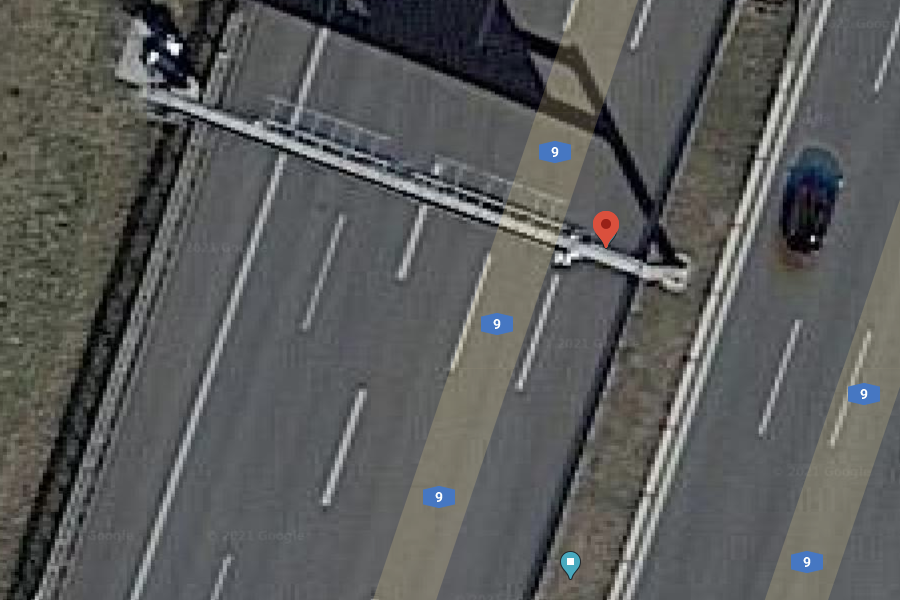
\includegraphics[width=0.45 \linewidth]{images/calibration/google_maps_s50_s.png} &
      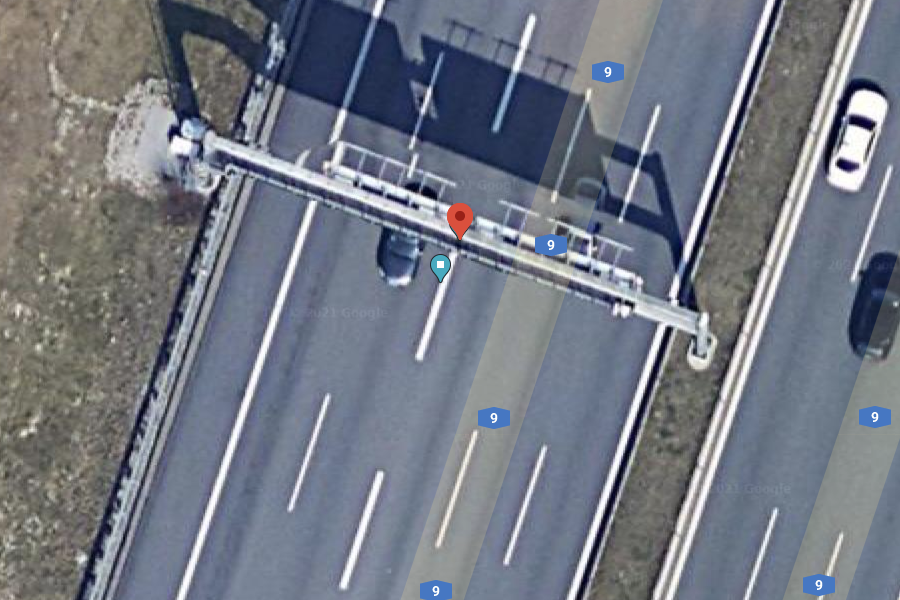
\includegraphics[width=0.45 \linewidth]{images/calibration/google_maps_s40_n.png} 
  \end{tabular}
  \caption{Left: The positions of the cameras \camsn{4} (red) and \camsf{4} (green) and their respective looking directions (yellow). 
  Right: The positions of the cameras \camsn{5} (red) and \camsf{5} (green) and their respective looking directions (yellow). 
  It displays that the rotation of the cameras is in a reasonable range so that the cameras look along the highway as expected. 
  Also the cameras are within reasonable translational bounds around their real world location as \autoref{sec:static_calibration_expectable_error} shows.
  }
  \label{fig:google_maps}
  \end{figure*}

The proposed pose estimation algorithm from \autoref{eq:static_calibration_error} converges to a pair of optimal translation $T$ and rotation $R$ values for the camera pose.
These $T, R$ values approximate the projection from the world objects to the pixels as described in \autoref{eq:static_calibration_reprojection}.

Using a maps provider we assured that the resulting values are within reasonable ranges and that there are no systematic errors in the optimization.
The results are displayed in \autoref{fig:google_maps}

\subsubsection{Points needed for convergence}
\label{sec:static_calibration_number_points}
The correspondences build up a system of linear equations. 
This system of equations is solvable if there exist a more or equal number of constraints on the parameters than there are degrees of freedoms in the system:
\begin{equation}
  \label{eq:static_calibration_reprojection_evaluation}
  p_c = \pi \left(  
    % \begin{bmatrix}
    %   R, T \\
    %   0, 1
    % \end{bmatrix} *
    R * T *
    (o_c + \lambda_c * h_c)
  \right), \forall c \in C
\end{equation}
This is the case if:
\begin{equation}
  \begin{split}
  2 * \left\lvert C \right\rvert \quad \geq& \quad 5 + 3 + 3 + 1 * \left\lvert C \right\rvert \\
  \left\lvert C \right\rvert \quad \geq& \quad 11 
\end{split}
\end{equation} 

As each of the pixel per correspondence gives us two constraints and we optimize over the 5 intrinsic parameters (\autoref{eq:static_calibration_intrinsic_parameters}), the 3 extrinsic translation, 3 extrinsic rotation parameters and one $\lambda$ parameter per correspondence.
We see that 11 points are enough to recover the pose.

\subsubsection{Structure of points}
The best result are shown when there are at least two correspondences per object.
These correspondences should be the top and bottom most visible pixel of the object.
If there exists only 1 or a low number of near pixels, the algorithm cannot precisely recover the camera pose, as it is free to move the correspondence along the center line of the object.
The algorithm therefore cannot distinguish the solutions where the camera is placed low, thus projecting a high point of an object to a low pixel correspondence, 
or if it should place the camera higher and lower the correspondences world position along the center line.

We thus conclude that the best solution is recovered the more the pixels fill the whole object, and the more spread to the top and bottom of the object the correspondences are. 




























\subsubsection{Expectable Error Bounds}
\label{sec:static_calibration_expectable_error}

Due to measurement uncertainty in the camera sensors we expect some remaining error after pose estimation.
To conclude a lower bound on this error we start from the optimized focal length $f_px$ in pixels and the sensor width $w_{mm}$ in millimeters and $w_{px}$ in pixels.

The focal length in millimeters is given by 
\begin{equation}
  f_{mm} = f_{px} * \frac{w_{mm}}{w_{px}}
\end{equation}

We then calculate the field of view (FOV) in radians by 
\begin{equation}
  FOV_x = 2 * \arctan \left(\frac{f_{mm}}{2 * w_{mm}}\right)
\end{equation} 
Equivalent the $FOV_y$ with the height of the sensor $h_{mm}$.

This brings us to a formulation for the angle spanned by each pixel
\begin{equation}
  \alpha_{px} = \frac{w_{px}}{FOV_x}
\end{equation} 

Using the pythagorean formula we can then calculate the uncertainty $u$ in meters of the camera as the spanned meters per pixel relative to the distance $d$ from the camera 
\begin{equation}
  u = \tan (\alpha_{px}) * d
\end{equation}

\begin{table}
  \begin{center}
    \begin{tabular}{ |c | c | c| c| c| c |}
      \hline
      Camera & $f_{px}$ & $FOV_x [^{\circ}]$ & $\alpha_{px}$ & $d [m]$ & $u [cm]$ \\
      \hline
      \camsf{4} & 8591 & 12.753 & $1.16e^{-4}$ & 200 & 2.32 \\
      \camsf{4} & 8591 & 12.753 & $1.16e^{-4}$ & 650 & 7.54 \\
      \hline
      \camsn{4} & 2735 & 38.678 & $3.52e^{-4}$ & 25 & 0.88 \\
      \camsn{4} & 2735 & 38.678 & $3.52e^{-4}$ & 450 & 15.82 \\
      \hline
      \camsf{5} & 8868 & 12.357 & $1.12e^{-4}$ & 200 & 2.22 \\
      \camsf{5} & 8868 & 12.357 & $1.12e^{-4}$ & 650 & 7.30 \\
      \hline
      \camsn{5} & 2747 & 38.527 & $3.50e^{-4}$ & 25 & 0.88\\
      \camsn{5} & 2747 & 38.527 & $3.50e^{-4}$ & 450 & 15.76 \\
      \hline
    \end{tabular}
  \end{center}
  \caption{
    \label{tab:static_calibration_camera_uncertainty}
  }
\end{table}

\autoref{tab:static_calibration_camera_uncertainty} displays the uncertainty for our cameras.
It shows that the far cameras cannot distinguish between points that are $\sim 2.2 cm$ at the nearest visible distance from the camera ranging up to $\sim 7.54 cm$ at the farthest distance.
The near cameras cannot distinguish between points that are $\sim 0.88 cm$ at the nearest visible distance from the camera ranging up to $\sim 15.82 cm$ at the farthest distance.

This gives a lower bound for the uncertainty in the translational parameters of the camera.
The camera translation cannot be more precise as the lowest uncertainty in the measurements.
Nonetheless, in practice the error will sum up and the translation parameters will drift inevitable. 

This concludes that objects near to the camera are more reliable to detect and to use for estimation.





















\subsubsection{Expectable Deviations among Estimations}
The proposed pose estimation algorithm is based on the minimization of the reprojection-error \autoref{eq:static_calibration_reprojection}.
As with all optimization problems convergence is reached when the values that are optimized don't change anymore.

The optimization jointly optimizes for the 6 camera parameters, 3 for the translation, 3 for the Euler angle rotation and one $\lambda$ parameter per correspondence.
The resulting high-dimensional problem exceeds multiple minima, whereas each represents a configuration for the camera pose that well explains the dependency between pixels, world objects and the camera. 

As stated previously the loss landscape does exhibit a multitude of local minima, thus the optimization procedure converges to different sets of parameters. 

\begin{figure}[t]
  \centering
  \begin{tabular}{cc}
    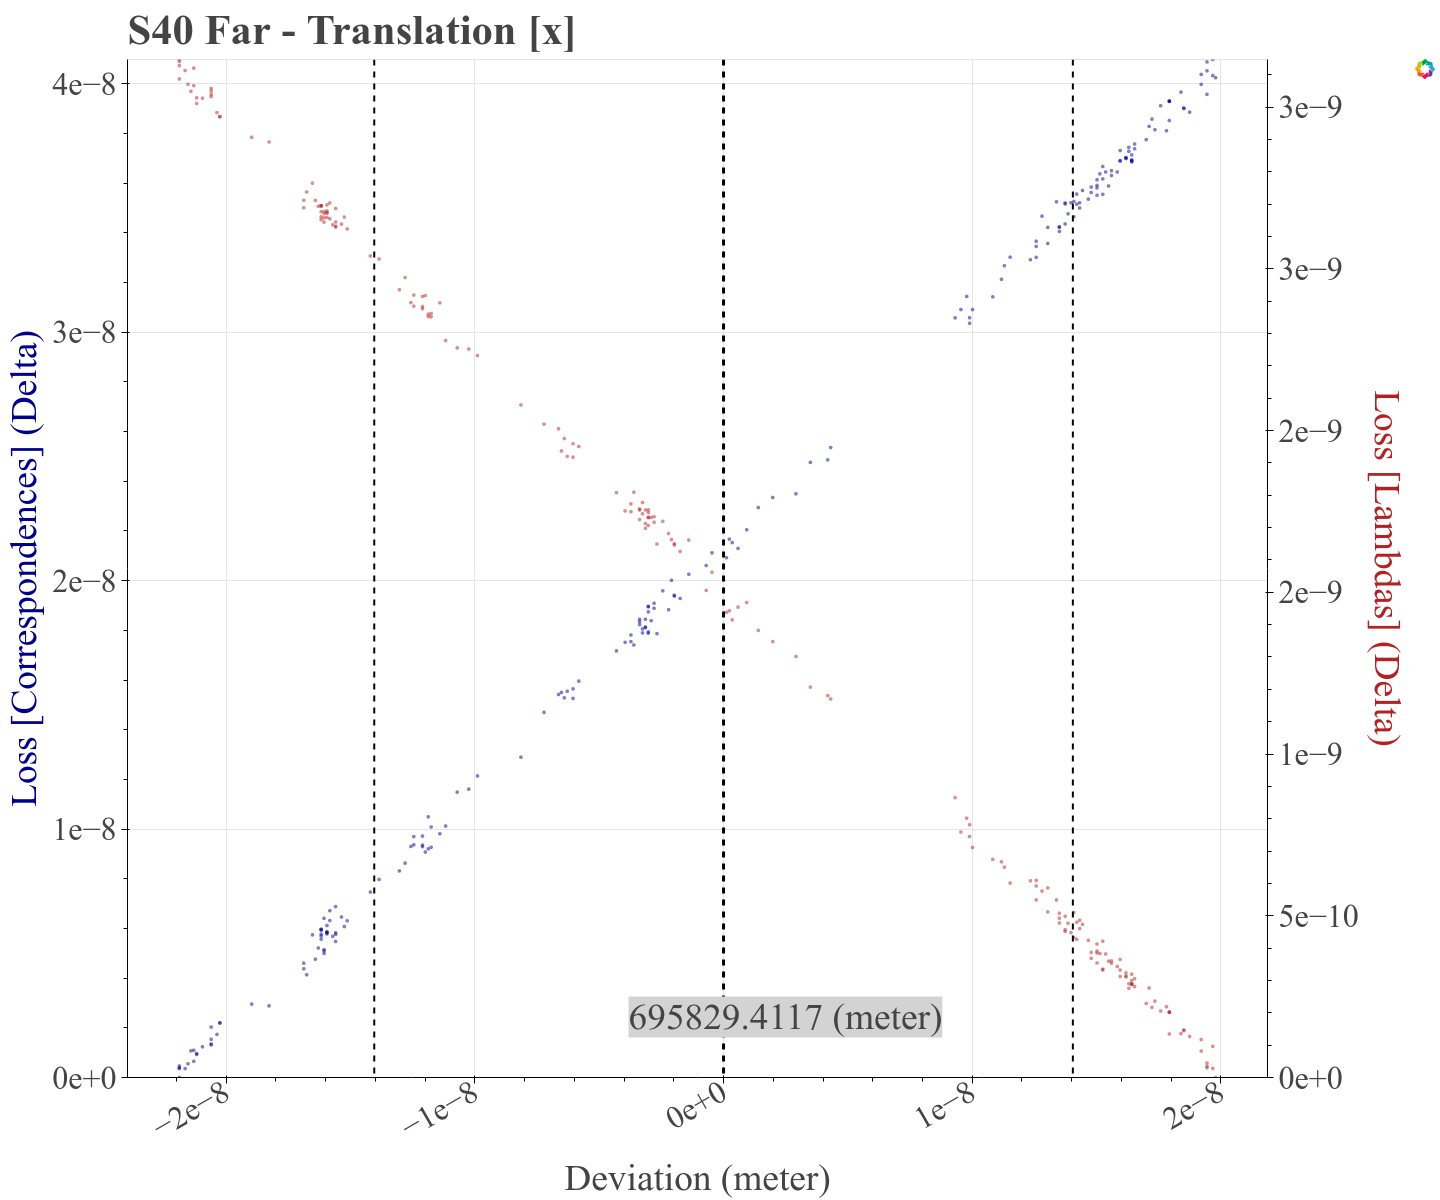
\includegraphics[width=0.45 \linewidth]{diagrams/calibration/s40_n_far/parameters.csv/Translation[x]_vs_Loss[Correspondences]_vs_Loss[Lambdas]_cluster_All.png} &
    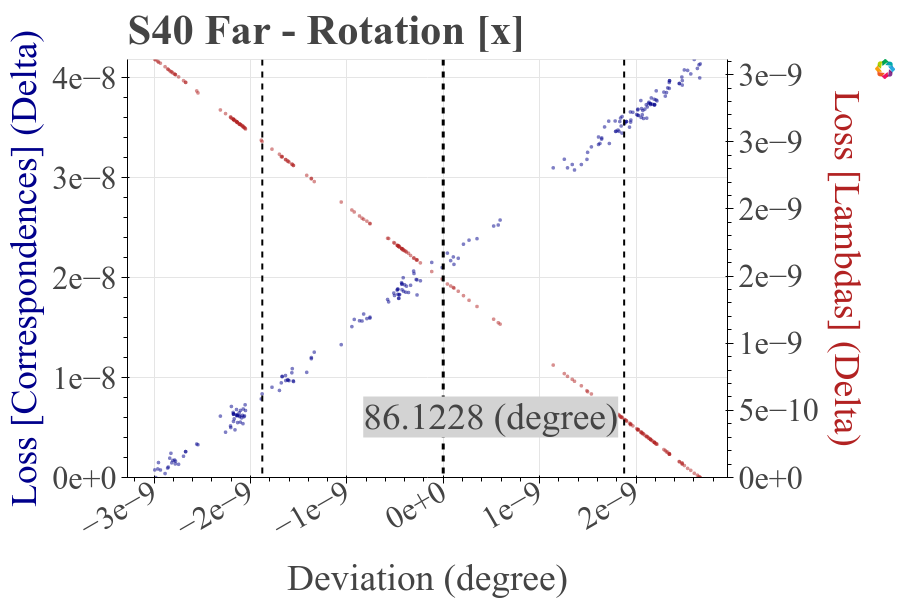
\includegraphics[width=0.45 \linewidth]{diagrams/calibration/s40_n_far/parameters.csv/Rotation[x]_vs_Loss[Correspondences]_vs_Loss[Lambdas]_cluster_All.png} \\
    
    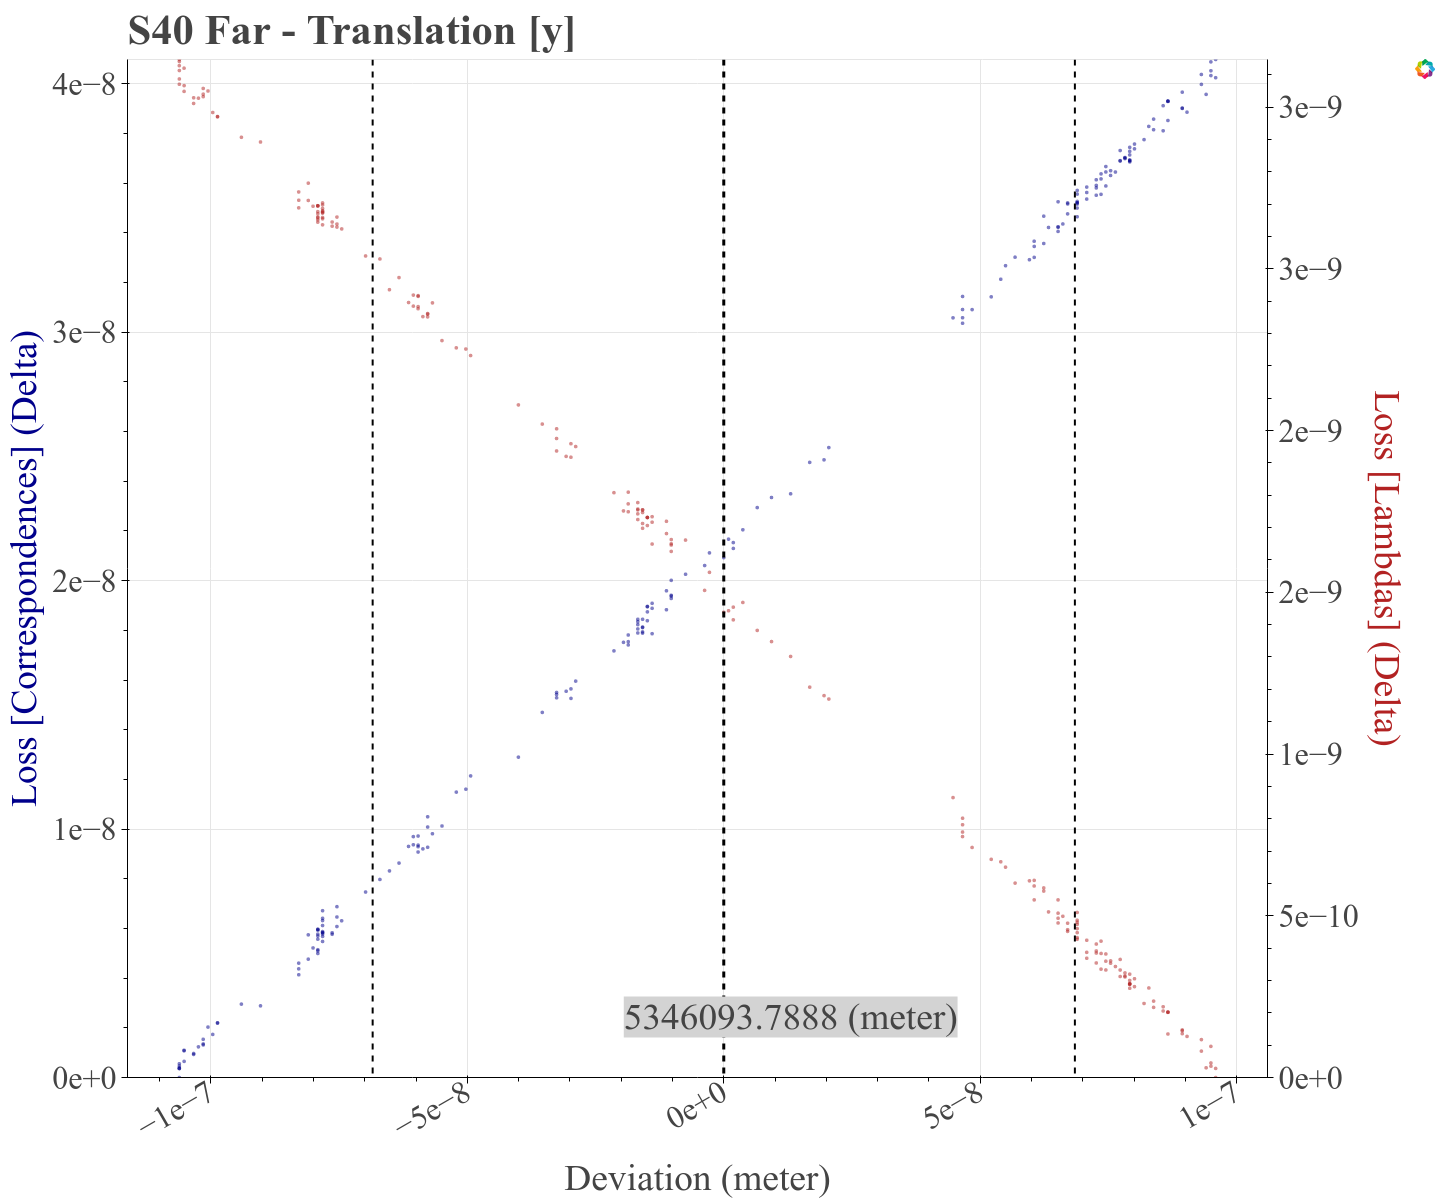
\includegraphics[width=0.45 \linewidth]{diagrams/calibration/s40_n_far/parameters.csv/Translation[y]_vs_Loss[Correspondences]_vs_Loss[Lambdas]_cluster_All.png} &
    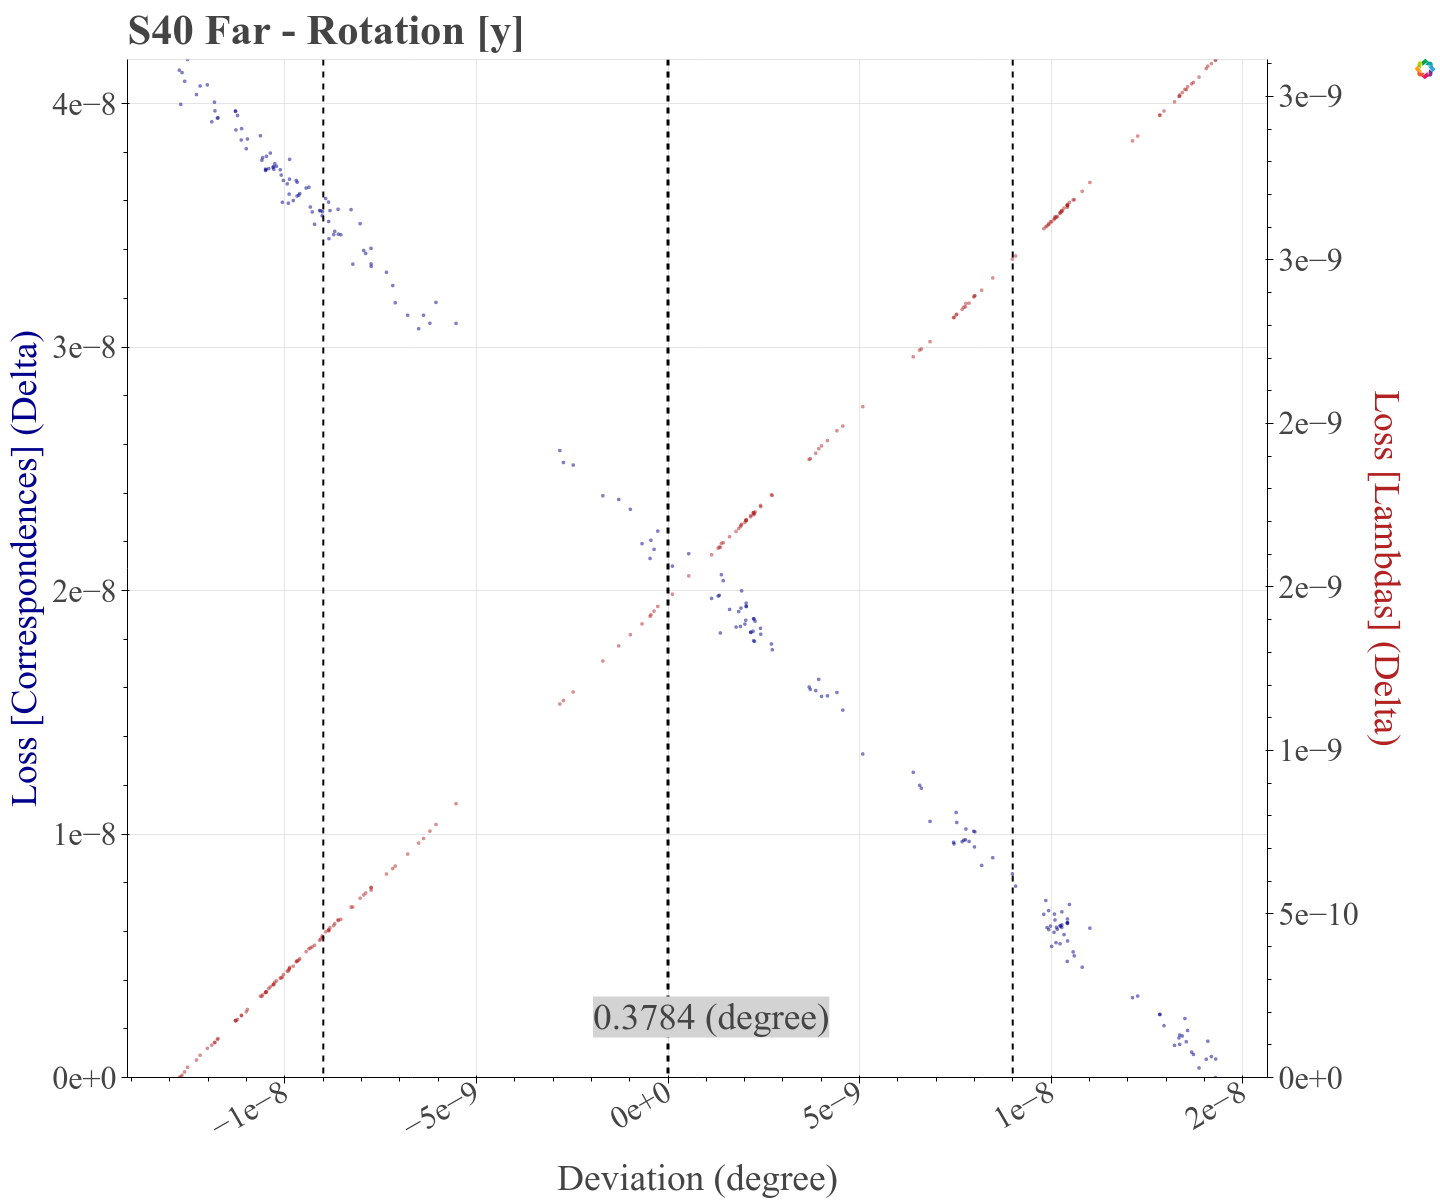
\includegraphics[width=0.45 \linewidth]{diagrams/calibration/s40_n_far/parameters.csv/Rotation[y]_vs_Loss[Correspondences]_vs_Loss[Lambdas]_cluster_All.png} \\
    
    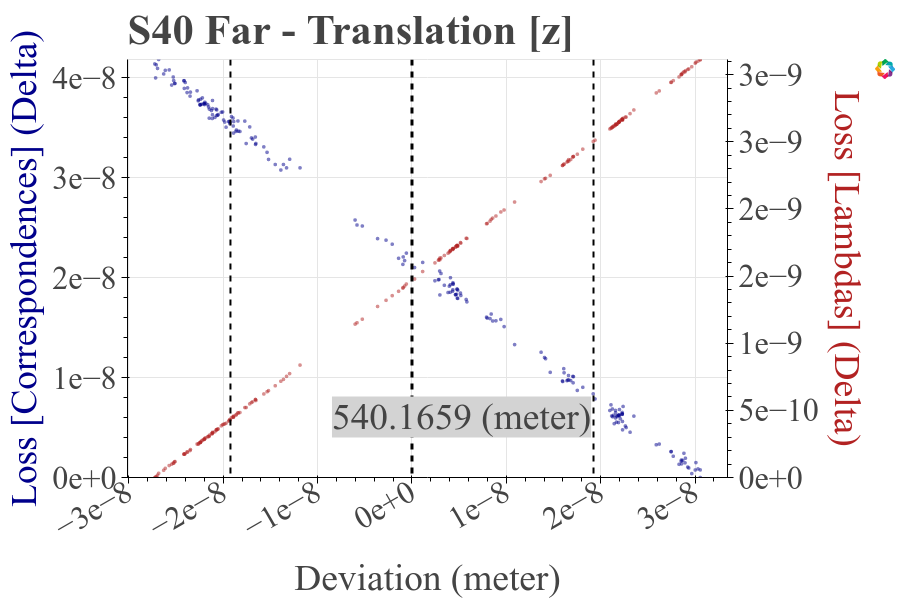
\includegraphics[width=0.45 \linewidth]{diagrams/calibration/s40_n_far/parameters.csv/Translation[z]_vs_Loss[Correspondences]_vs_Loss[Lambdas]_cluster_All.png} &
    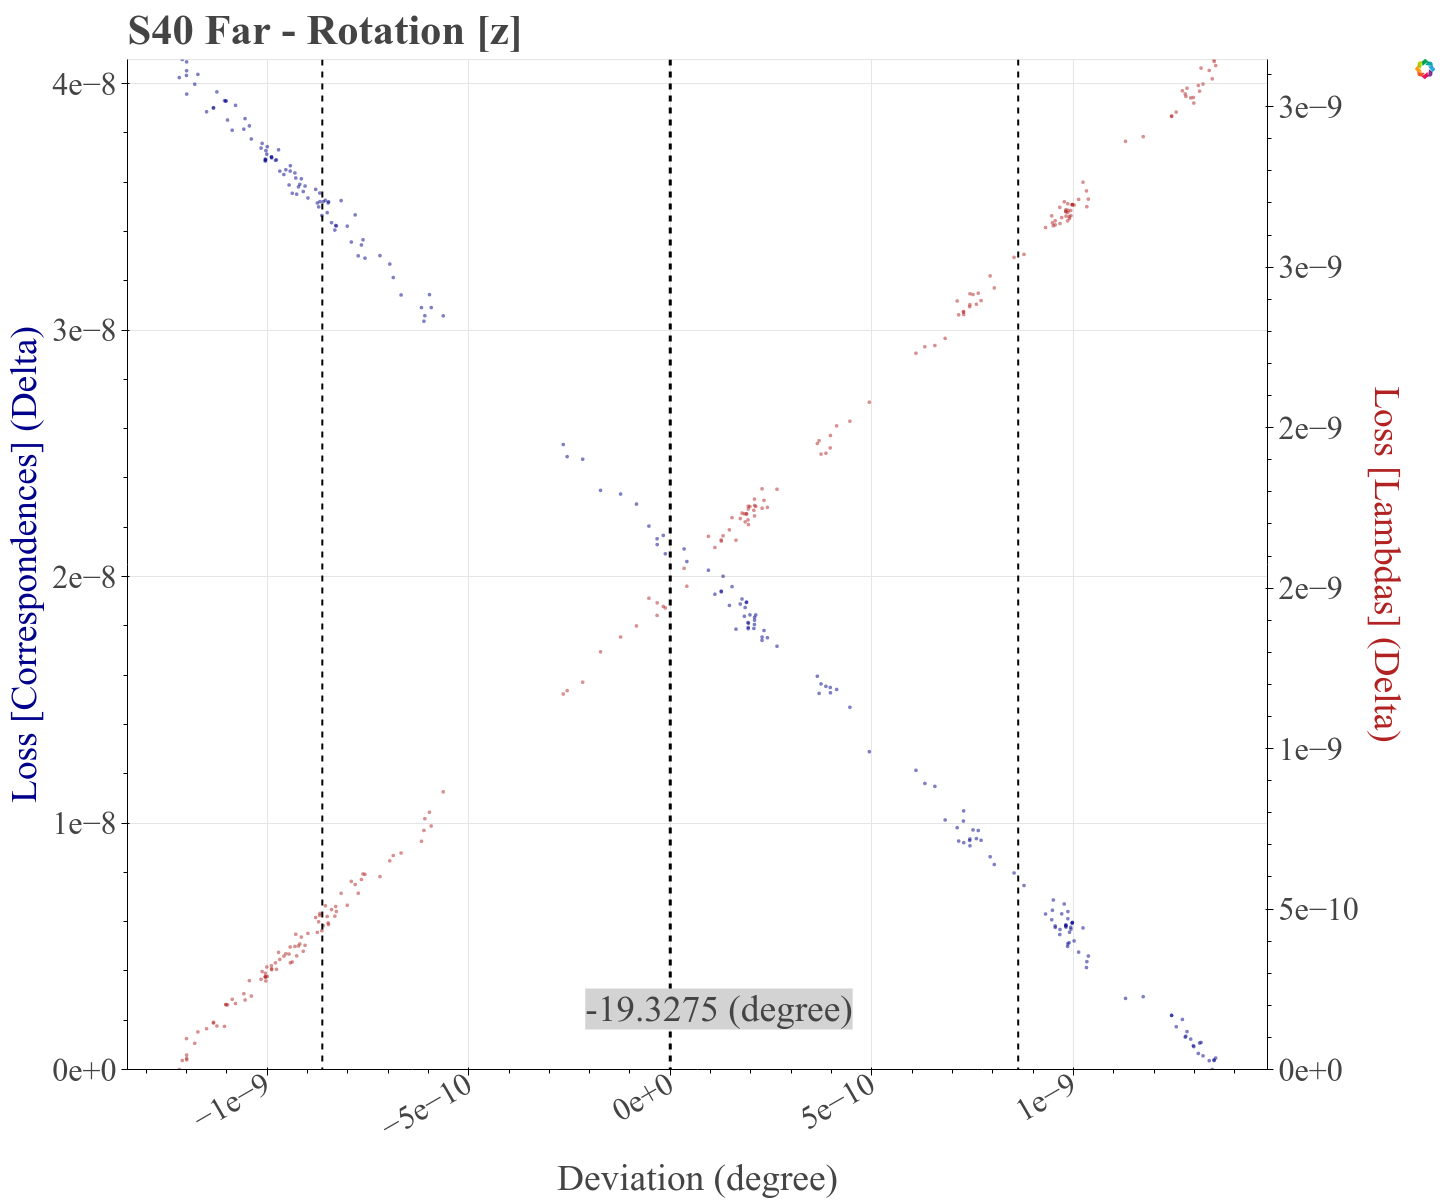
\includegraphics[width=0.45 \linewidth]{diagrams/calibration/s40_n_far/parameters.csv/Rotation[z]_vs_Loss[Correspondences]_vs_Loss[Lambdas]_cluster_All.png} \\

    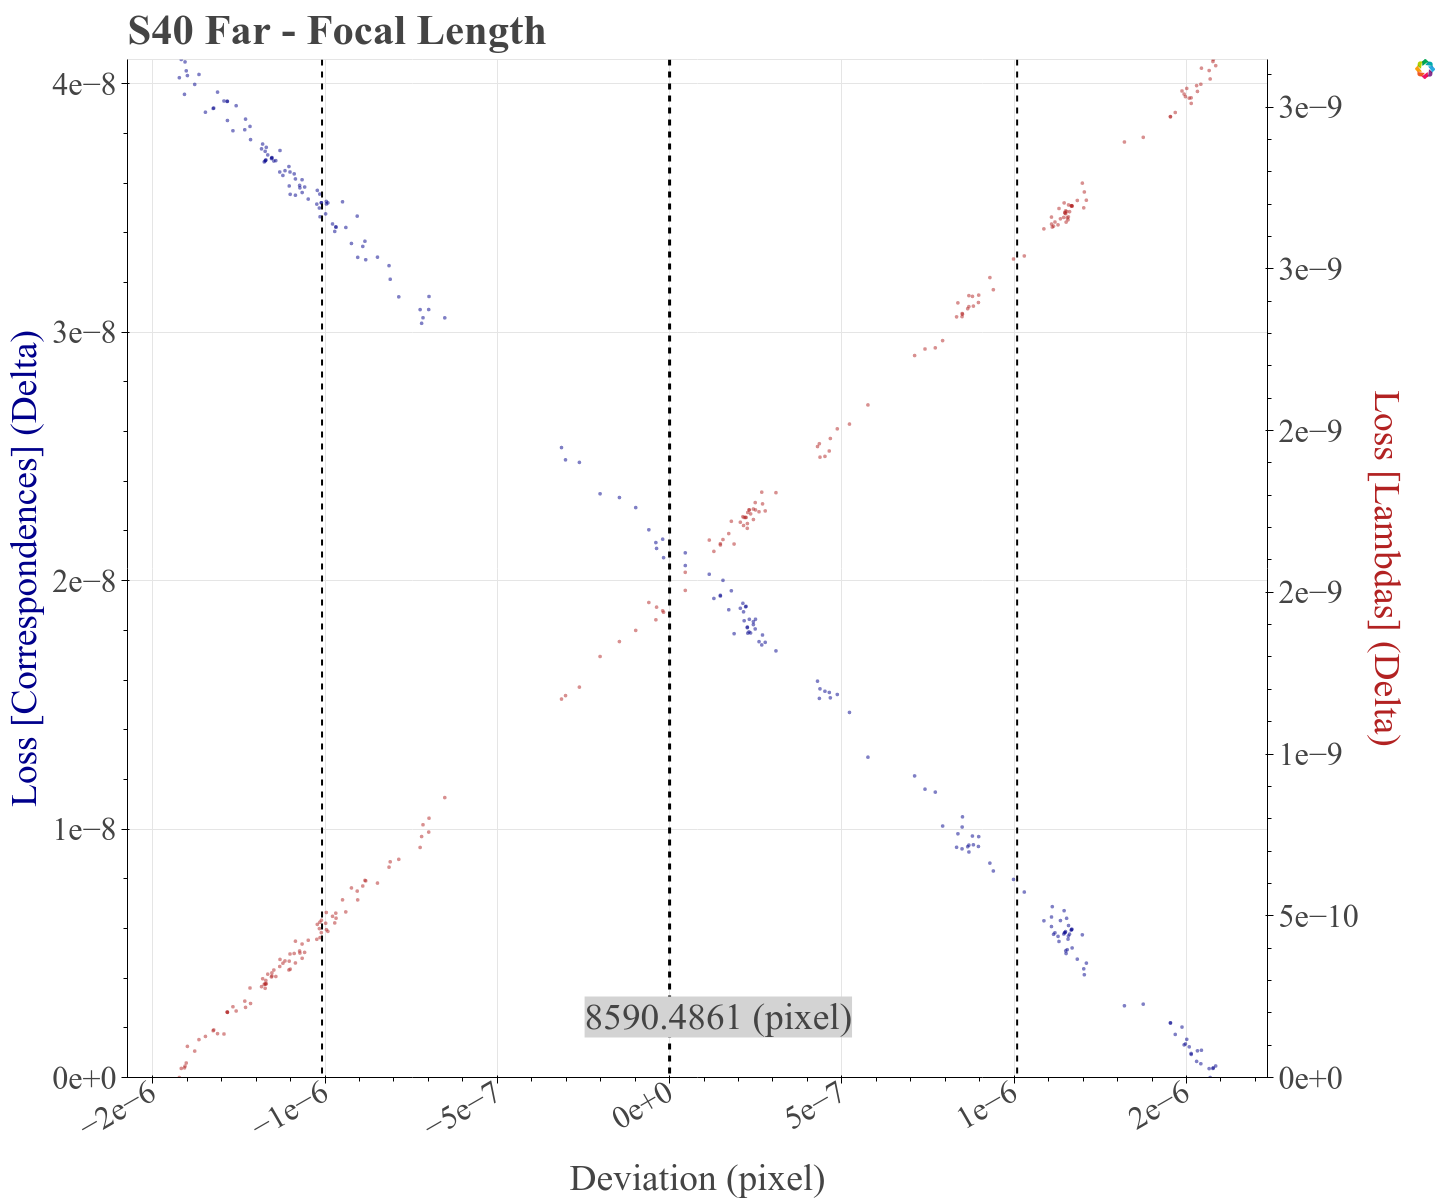
\includegraphics[width=0.45 \linewidth]{diagrams/calibration/s40_n_far/parameters.csv/FocalLength_vs_Loss[Correspondences]_vs_Loss[Lambdas]_cluster_All.png} \\
\end{tabular}
\caption{
  Left: The resulting translational parameters plotted against the remaining losses. 
  Right: The resulting rotational parameters plotted against the remaining losses.
  The mean of the distributions is displayed as thick dashed line. The smaller dashed lines display the standard deviation $\sigma$.
  The $\sigma$ of the translations does not exceed $2 * 10^{-4} m = 0.2 mm$.
  For the rotation $\sigma$ is at most $4 * 10^{-4} deg$.
  }
\label{fig:static_calibration_algorithmic_error}
\end{figure}

\autoref{fig:static_calibration_algorithmic_error} displays the resulting parameters for the camera \camsf{4}.
We plot the loss of the correspondence residuals and the $\lambda$ residual blocks against each of the parameters.
The translation parameters are in meters and relative to the transverse mercator projection \cite{lambert1894anmerkungen}.
The rotation parameters are in degree of Euler angles.

The plots show that the standard deviation $\sigma$ of the translations does not exceed $2 * 10^{-4} m = 0.2 mm$.
For the rotation $\sigma$ is at most $4 * 10^{-4} deg$. 

We have shown the expectable error for the parameters resulting from the sensor and map inaccuracies in \autoref{sec:static_calibration_expectable_error}. 
We conclude that in relation to these the algorithmic error can be neglected.

In the appendix \autoref{sec:appendix} we additionally evaluate the other cameras.

% \subsubsection{Minimal number of correspondences}
